% Konfigurationsdatei f\"ur die Pfaddefinitionen einlesen
%  se-wa-pfade.tex
%
%
%  J\"org Baumgart
%  2012-12-20
%  
%  Pfaddefinitionen (Ordnerdefinitionen) f\"ur das Einlesen von
%  -- .sty-Dateien und
%  -- Textbaustenen f\"ur die Hinweise zur Verwendung von LaTeX
%  -- jpg-Bildern
%
\newcommand{\seWaPathSty}{se-wa-styles}
\newcommand{\seWaPathText}{se-wa-textbausteine-vorlagen}
\newcommand{\seWaPathJpg}{se-wa-jpg}

%
%
% Festlegung der Sprache: 
\newcommand{\seWaSprache}{deutsch}
%\newcommand{\seWaSprache}{englisch}


%
% Einlesen der .sty-Dateien
%
%  se-wa-input-styles-v095.tex
%
%  Joerg Baumgart 01.08.2011
%
%  Zusammenfassung und Konfiguration wichtiger Styles f\"ur die 
%  Erzeugung von Seminar-, Projekt- und Bachelorarbeiten
%
%  2012-03-12: auf Version 0.94 umgestellt
%
%
% 2012-12-13: auf Version 0.95 umgestellt
%                     Sprachoptionen englisch/deutsch zusammengef\"uhrt
%                     bchart.sty hinzugenommen
%                 
%


\documentclass[12pt,BCOR=10mm,headinclude=on,footinclude=off,bibliography=totoc]{scrreprt}
\usepackage[T1]{fontenc}
\usepackage[latin1]{inputenc}
\usepackage{ifthen}
% 2012-12-13
\ifthenelse{\equal{\seWaSprache}{deutsch}}{% Deutsche Einstellungen
\usepackage[ngerman]{babel}% 
}{% Englische Einstellungen
\usepackage[english]{babel}% 
}

\usepackage{lmodern}

\usepackage{tikz} % Graphikpaket, das zu pdfLaTeX kompatibel ist
\usepackage{xkeyval} % Definition von Kommandos mit mehreren optionalen Argumenten
\usepackage{listings} % Formatierung von Programmlistings
\usepackage{graphicx} % Einbinden von Graphiken
\usepackage{color}
\usepackage{\seWaPathSty/slashbox} % Diagonalen in Tabellenfeldern
\usepackage{framed} % Erzeugung schwarzer Linien am linken Rand zur Hervorhebung von Textteilen
\usepackage{caption} % Korrektes Setzen einer mehrzeiligen float-Unterschrift bei neu definierten float-Umgebungen
\usepackage{floatrow}
% 2012-12-13
\usepackage{\seWaPathSty/bchart} % Kommandos zur Erzeugung von Balkendiagrammen


% Es wird jeweils die sty-Datei importiert und entsprechende Konfigurationseinstellungen werden vorgenommen

\usepackage{\seWaPathSty/se-jb-scrpage2} % Formatierung der Kopf- und Fu{\ss}zeilen
\usepackage{\seWaPathSty/se-jb-footmisc}    % Fussnoten besser formatieren

\usepackage{\seWaPathSty/se-jb-glossaries-v094} % Abk\"urzungsverzeichnis, Symbolverzeichnis, Glossar
   
\usepackage{\seWaPathSty/se-jb-floatrow}    % Definition und Konfiguration von float-Umgebungen (figure, table, die neue programm-Umgebung)
% Achtung: se-jb-varioref muss nach se-jb-floatrow importiert werden; 
% andernfalls ist der counter programm f\"ur die labelformat-Anweisung noch nicht definiert   
\usepackage{\seWaPathSty/se-jb-varioref}   % Definition von Querverweisen
\usepackage{\seWaPathSty/se-jb-chngcntr}   % Kapitelweise oder globale Nummerierung von Abbildungen etc.
   
\usepackage{\seWaPathSty/se-jb-listen} % Definition neuer, besser formatierter Listen
\usepackage{\seWaPathSty/se-jb-kommandos-v095} % neue Kommandos f\"ur Seminar-, Projekt- und Bachelorarbeiten
% 2012-12-13
\ifthenelse{\equal{\seWaSprache}{englisch}}{\usepackage{\seWaPathSty/se-jb-kommandos-englisch}}{}

%
% Individuelle Konfiguration des Dokumentes
%
%  Individuelle Konfiguration einer Projektarbeit/Bachelorarbeit
%
%
%
%

% 2012-10-27
%
% \"Anderung des Schrifttyps f\"ur das gesamte Dokument
%
% Das gesamte Dokument wird in einer serifenlosen Schrift gesetzt
%\renewcommand{\familydefault}{\sfdefault}
%
% Das gesamte Dokument wird in einer Serifenschrift gesetzt
% Achtung: serifenlose Schriften sind jetzt grunds\"atzlich nicht mehr nutzbar!
%
%\renewcommand{\sffamily}{\normalfont}

% 2012-12-05
%
% Verwendung des url-Pakets
% Durch den optionalen Paremeter hyphens wird eine Trennung 
% von URLs auch nach Bindestrichen erlaubt
\usepackage[hyphens]{url}


% 2012-10-27
%
%
% Literaturverzeichnis
% 
% Literaturverzeichnis gem\"ass den Vorgaben von Theisen aufbauen
\usepackage{\seWaPathSty/se-jb-jurabib-theisen} 
% Verwendung der Harvard-Zitierweise
%\usepackage{\seWaPathSty/se-jb-jurabib-harvard} 

% Weitere Optionseinstellungen f\"ur das Koma-Script
%
% Zwischen Abs\"atzen einen Abstand von 0.5 \baselineskip erzeugen
\KOMAoption{parskip}{full}
%
% Vergleiche Duden "Gliederung von Nummern, S.111" 
% DIN 5008 anschauen, wenn sie neu ver\"offentlicht wurde
\KOMAoption{numbers}{noendperiod}
%
%



%  Voreinstellungen f\"ur floats
%  Durch die verwendeten Parameter wird die Wahrscheinlichkeit deutlich kleiner, 
%  dass Gleitobjekte (z. B. Abbildungen) ans Ende des Dokumentes verschoben 
%  werden; 
%  Achtung: clearpage erzwingt die Ausgabe von Gleitobjekten
%
\renewcommand{\topfraction}{1}  % Gleitobjekte d\"urfen eine Seite zu 100% belegen 
\renewcommand{\bottomfraction}{1} % Entsprechender Wert f\"ur den unteren Teil der Seite
\renewcommand{\textfraction}{0} % Eine Seite darf auch ohne Fliesstext existieren
%%%\renewcommand{\floatpagefraction}{1} % Bedeutung unklar, daher keine Ver\"anderung des Vorgabewertes 
                                                                        % von 0.5; eventuell bringt ein \"Anderung auf 1 etwas, wenn 
                                                                         % Probleme mit floats auftreten
                                                                         
                                                                         
                                                                         
% Konfiguration von Programm-Listings
% 
% Achtung: hier gibt es nahezu beliebig viele weitere Konfigurationm\"oglichkeiten; vgl. Paketdokumentation
%
\lstset{language=Java,basicstyle=\ttfamily,keywordstyle=\color{blue},captionpos=b,aboveskip=0mm,belowskip=0mm,
          xleftmargin=0em}               
          
%
% Grundkonfiguration der Abs\"ande zwischen den Items der maximal f\"unf Verschachtelungsebenen der 
% neuen Listenumgebungen
%                                                                             
% Initialisierung der Abst\"ande zwischen den items f\"ur seList; Grundeinheit: 0.5\baselineskip; siehe se-jb-listen
\seSetlistbaselineskip{1}{0.75}{0.75}{0.75}{0.75}
% Initialisierung der Abst\"ande zwischen den items f\"ur seToplist; Grundeinheit: 0.5\baselineskip; siehe se-jb-listen
\seSettoplistbaselineskip{1}{0.75}{0.75}{0.75}{0.75}     


% Einlesen der sprachabh\"angigen Konfigurationsdatei
%
%
\ifthenelse{\equal{\seWaSprache}{deutsch}}{% deutsch
% wa-konfiguration-deutsch
%
% 2012-12-13
% 
% Diese Datei wird f\"ur die Sprachoption deutsch verwendet, d. h.  
% \newcommand{\seWaSprache}{deutsch}
%
%
% In dieser Datei k\"onnen Neudefinitionen vorgenommen werden f\"ur:
% -- Verzeichnisse
% -- Unter-/\"Uberschriften von Abbildungen, Tabellen und Listings
% -- Querverweise innerhalb des Textes

%
%  Konfiguration der verschiedenen Verzeichnisse
%
%  abstandEintrag: Wert wird mit \baselineskip multipliziert
%

%
%  Abbildungsverzeichnis
%
\seKonfigurationAbb[
%verzeichnisname=Abbildungsverzeichnis,
labeltextLinks=, % kein Text links;
%labeltextRechts=:,
labelbreite=1cm,
%labeleinzug=1cm,
%abstandEintrag=1,
%newpage=ja,
%pnumwidth=20mm,
%dotsep=1000,
%tocrmarg=4.5cm,
%abstandVerzeichnis=-1mm
]

%
% LIstingverzeichnis
%
\seKonfigurationPrg[
%verzeichnisname=Listing-Verzeichnis,
labeltextLinks=,
%labeltextRechts=:,
labelbreite=1cm,
%labeleinzug=2cm,
%abstandEintrag=1,
%newpage=ja,
%pnumwidth=20mm,
%dotsep=1000,
%tocrmarg=4.5cm,
%abstandVerzeichnis=-10mm
]

%
% Tabellenverzeichnis
%
\seKonfigurationTab[
%verzeichnisname=Liste der Tabellen,
labeltextLinks=,
%labeltextRechts=:,
labelbreite=1cm,
%labeleinzug=0.5cm,
%abstandEintrag=1,
%newpage=ja,
%pnumwidth=20mm,
%dotsep=1000,
%tocrmarg=4.5cm,
%abstandVerzeichnis=-10mm
]

%
% Abk\"urzungsverzeichnis
%
\seKonfigurationAbk[
%verzeichnisname=Liste der Abk\"urzungen,
%labelbreite=3cm,
%labeleinzug=0.5cm,
%abstandEintrag=1,
%newpage=ja,
%abstandVerzeichnis=-10mm
]

%
% Symbolverzeichnis
% 
\seKonfigurationSym[
%verzeichnisname=Liste der Symbole,
%labelbreite=4cm,
%labeleinzug=3.5cm,
%abstandEintrag=1,
%newpage=ja,
%abstandVerzeichnis=-10mm
]

%
% Glossar
%
\seKonfigurationGlo[
%verzeichnisname=Glossar,
%abstandEintrag=0,
]



% (eventuelle) Neudefinition f\"ur die Unter-/\"Uberschriften von Abbildungen, Tabellen und Listings
%
%
%\renewcommand{\seCaptionNameAbbildung}{Abb.}
%\renewcommand{\seCaptionNameTabelle}{Tab.}
%\renewcommand{\seCaptionNameProgramm}{Prg.}


% % (eventuelle) Neudefinition f\"ur Querverweise innerhalb des Textes
%
%
%
%\renewcommand{\seQuerverweisSeite}{Seite}
%\renewcommand{\seQuerverweisAbbildung}{Abb.}
%\renewcommand{\seQuerverweisTabelle}{Tab.}
%\renewcommand{\seQuerverweisProgramm}{Prg.}
%\renewcommand{\seQuerverweisGleichung}{Gl.}
%
\renewcommand{\seQuerverweisChapter}{Kapitel}
\renewcommand{\seQuerverweisSection}{Kapitel}
\renewcommand{\seQuerverweisSubsection}{Kapitel}
\renewcommand{\seQuerverweisSubsubsection}{Kapitel}
\renewcommand{\seQuerverweisParagraph}{Kapitel}


%
% Kommandos f\"ur die Konfiguration von URL-Eintr\"agen im Literaturverzeichnis
%
\renewcommand*{\biburlprefix}{\jblangle{}URL: }
\renewcommand*{\biburlsuffix}{\jbrangle{}}
\renewcommand*{\bibbudcsep}{ -- }
\AddTo\bibsgerman{\renewcommand*{\urldatecomment}{Zugriff am }}


%
}{% englisch
% wa-konfiguration-englisch
%
% 2012-12-13
% 
% Diese Datei wird f\"ur die Sprachoption englisch verwendet, d. h.  
% \newcommand{\seWaSprache}{englisch}
%
%
% In dieser Datei k\"onnen Neudefinitionen vorgenommen werden f\"ur:
% -- Verzeichnisse
% -- Unter-/\"Uberschriften von Abbildungen, Tabellen und Listings
% -- Querverweise innerhalb des Textes

%
%  Konfiguration der verschiedenen Verzeichnisse
%
%  abstandEintrag: Wert wird mit \baselineskip multipliziert
%

%
%  Abbildungsverzeichnis
%
\seKonfigurationAbb[
verzeichnisname=List of Figures,
labeltextLinks=, % kein Text links;
%labeltextRechts=:,
labelbreite=1cm,
%labeleinzug=1cm,
%abstandEintrag=1,
%newpage=ja,
%pnumwidth=20mm,
%dotsep=1000,
%tocrmarg=4.5cm,
%abstandVerzeichnis=-1mm
]

%
% LIstingverzeichnis
%
\seKonfigurationPrg[
verzeichnisname=List of Program Listings,
labeltextLinks=,
%labeltextRechts=:,
labelbreite=1cm,
%labeleinzug=2cm,
%abstandEintrag=1,
%newpage=ja,
%%pnumwidth=20mm,
%dotsep=1000,
%tocrmarg=4.5cm,
%abstandVerzeichnis=-10mm
]

%
% Tabellenverzeichnis
%
\seKonfigurationTab[
verzeichnisname=List of Tables,
labeltextLinks=,
%labeltextRechts=:,
labelbreite=1cm,
%labeleinzug=0.5cm,
%abstandEintrag=1,
%newpage=ja,
%pnumwidth=20mm,
%dotsep=1000,
%tocrmarg=4.5cm,
%abstandVerzeichnis=-10mm
]

%
% Abk\"urzungsverzeichnis
%
\seKonfigurationAbk[
verzeichnisname=List of Abbreviations,
%labelbreite=3cm,
%labeleinzug=0.5cm,
%abstandEintrag=1,
%newpage=ja,
%abstandVerzeichnis=-10mm
]

%
% Symbolverzeichnis
% 
\seKonfigurationSym[
verzeichnisname=List of Symbols,
%labelbreite=4cm,
%labeleinzug=3.5cm,
%abstandEintrag=1,
%newpage=ja,
%abstandVerzeichnis=-10mm
]

%
% Glossar
%
\seKonfigurationGlo[
verzeichnisname=Glossary,
%abstandEintrag=0,
]



% (eventuelle) Neudefinition f\"ur die Unter-/\"Uberschriften von Abbildungen, Tabellen und Listings
%
%
\renewcommand{\seCaptionNameAbbildung}{Figure}
\renewcommand{\seCaptionNameTabelle}{Table}
\renewcommand{\seCaptionNameProgramm}{Listing}


% % (eventuelle) Neudefinition f\"ur Querverweise innerhalb des Textes
%
%
%
\renewcommand{\seQuerverweisSeite}{page}
\renewcommand{\seQuerverweisAbbildung}{figure}
\renewcommand{\seQuerverweisTabelle}{table}
\renewcommand{\seQuerverweisProgramm}{listing}
\renewcommand{\seQuerverweisGleichung}{equation}
%
\renewcommand{\seQuerverweisChapter}{chapter}
\renewcommand{\seQuerverweisSection}{chapter}
\renewcommand{\seQuerverweisSubsection}{chapter}
\renewcommand{\seQuerverweisSubsubsection}{chapter}
\renewcommand{\seQuerverweisParagraph}{chapter}


%
% Kommandos f\"ur die Konfiguration von URL-Eintr\"agen im Literaturverzeichnis
%
\renewcommand*{\biburlprefix}{\jblangle{}URL: }
\renewcommand*{\biburlsuffix}{\jbrangle{}}
\renewcommand*{\bibbudcsep}{ -- }
\AddTo\bibsenglish{\renewcommand*{\urldatecomment}{visited on }}


}

% Kommandos, die direkt nach \begin{document} ausgef\"uhrt werden m\"ussen
%
%
%
\AtBeginDocument{%
\renewcommand{\listfigurename}{\seAbbildungenVerzeichnisname}
\renewcommand{\listtablename}{\seTabellenVerzeichnisname}
\renewcommand{\figurename}{\seCaptionNameAbbildung}
\renewcommand{\tablename}{\seCaptionNameTabelle}
\pagenumbering{roman}
}
                                                              
                                                                         
%
% Definition von Abk\"urzungen, Symbolen und eventuell Glossareintr\"agen
%
% 2012-03-22 Verwendung des optionalen Parameters f\"ur die Pluralform einer Abk\"urzung
%
% 2012-02-06 Umstellung auf die neuen Kommandos
%
%
%
%  J\"org Baumgart
%  Definition einiger Abk\"urzungen
%  


% Definition von Abk\"urzungen
%
% 1. Parameter: Schluessel (key) der Abkuerzung
% 2. Parameter: Abkuerzung
% 3. Parameter: Vollform
% 4. Parameter: Vollform im Plural (optional; falls nicht definiert, wird der Wert des dritten Parameters verwendet)
%
\seNewAcronymEntry{dm}{DM}{Diagonalmatrix}{Diagonalmatrizen}

\seNewAcronymEntry{dhbw}{DHBW}{Duale Hochschule Baden-W\"urttemberg}{}{}

\seNewAcronymEntry{usb}{USB}{Universal Serial Bus}{}

\seNewAcronymEntry{ctan}{CTAN}{Comprehensive \TeX{} Archive Network}{}


% 2012-03-24
% \"Uber den optionalen Parameter in eckigen Klammern wird die Pluralform f\"ur das erste 
% Auftreten der Abk\"urzung definiert

\seNewAcronymEntry[URLs]{url}{URL}{Uniform Resource Locator}%
{Uniform Resource Locators}


% Definition von Symbolen
%
% 1. Parameter: Schluessel (key) des Symbols
% 2. Parameter: Symbol
% 3. Parameter: Text, der die Sortierreihenfolge festlegt (optional; falls nicht definiert, wird der Wert des zweiten 
%                        Parameters verwendet)
% 4. Parameter: Beschreibung des Symbols
%

\seNewSymbolEntry{ND}{ND}{a}{Nutzungsdauer einer Maschine}

\seNewSymbolEntry{pi}{$\pi$}{b}{Die Kreiszahl}




% Definition von Glossareintraegen
%
% 1. Parameter: Schluessel (key) des Glossareintrags
% 2. Parameter: Begriff, der im Glossar definiert wird
% 3. Parameter: Pluralform des Begriffes (optional; falls nicht definiert, wird der Wert des zweiten Parameters verwendet)
%                        Achtung: Pluralform gilt nur fuer das erste Auftreten des Begriffes im Text
% 4. Parameter: Beschreibung des Glossareintrags
%
%
%

\seNewGlossaryEntry{glos:AD}{Active Directory}{Active Directories}
{Active Directory ist in einem Windows 2000/Windows
Server 2003-Netzwerk der Verzeichnisdienst, der die zentrale
Organisation und Verwaltung aller Netzwerkressourcen erlaubt. Es
erm\"oglicht den Benutzern \"uber eine einzige zentrale Anmeldung den
Zugriff auf alle Ressourcen und den Administratoren die zentral
organisierte Verwaltung, transparent von der Netzwerktopologie und
den eingesetzten Netzwerkprotokollen. Das daf\"ur ben\"otigte
Betriebssystem ist entweder Windows 2000 Server oder
Windows Server 2003, welches auf dem zentralen
Dom\"anencontroller installiert wird. Dieser h\"alt alle Daten des
Active Directory vor, wie z.\,B. Benutzernamen und
Kennw\"orter.\protect\seFootcite{Vgl.}{S. 200}{Dud09}}


\seNewGlossaryEntry{glos:bs}{Betriebssystem}{Betriebssysteme}{Die Begriffsdefinition sollten Sie eigentlich kennen!}


% Definition von Glossareintraegen, die gleichzeitig im Abk�rzungsverzeichnis auftreten
%
% 1. Parameter: Schluessel (key) des Glossareintrags
% 2. Parameter: Abk\"urzung
% 3. Parameter: Vollform
% 4. Parameter: Vollform im Plural (optional; falls nicht definiert, wird der Wert des dritten Parameters verwendet)
% 5. Parameter: Beschreibung des Glossareintrags

\seNewAcronymGlossaryEntry{glos:ma}{MA}{Mobile Applikation}{Mobile Applikationen}
{Eine Applikation, die auf einem mobilen Endger\"at ausgef\"uhrt wird.}

% 2012-03-24
% \"Uber den optionalen Parameter in eckigen Klammern wird die Pluralform f\"ur die Abk\"urzung definiert

\seNewAcronymGlossaryEntry[TAen]{glos:ta}{TA}{Transaktion}%
{Transaktionen}%
{Was eine Transaktion ist, sollten Sie ebenfalls bereits wissen!}





% Alternative Definition von Abk\"urzungen; diese sollten nicht verwendet werden!!!
%
%\newacronym{dhbw}{DHBW}{Duale Hochschule Baden-W\"urttemberg}
%\newacronym{usb}{USB}{Universal Serial Bus}


% Alternative Definition von Symbolen
%
% Achtung: ohne sort wird nach Name sortiert
%\newglossaryentry{pi}{
%name=$\pi$,
%description={Die Kreiszahl},
%type=symbolslist,
%sort=b
%}
%
%\newglossaryentry{ND}{
%name=$\mbox{\textsl{ND}}$,
%description={Nutzungsdauer einer Maschine},
%type=symbolslist,%
%sort=a
%}



% Alternative Definition von Glossareintr\"agen
%
%\newglossaryentry{glos:AD}{
%first=Active Directory\textsuperscript{GL},
%name=Active Directory,
%description={Active Directory ist in einem Windows 2000/Windows
%Server 2003-Netzwerk der Verzeichnisdienst, der die zentrale
%Organisation und Verwaltung aller Netzwerkressourcen erlaubt. Es
%erm\"oglicht den Benutzern \"uber eine einzige zentrale Anmeldung den
%Zugriff auf alle Ressourcen und den Administratoren die zentral
%organisierte Verwaltung, transparent von der Netzwerktopologie und
%den eingesetzten Netzwerkprotokollen. Das daf\"ur ben\"otigte
%Betriebssystem ist entweder Windows 2000 Server oder
%Windows Server 2003, welches auf dem zentralen
%Dom\"anencontroller installiert wird. Dieser h\"alt alle Daten des
%Active Directory vor, wie z.\,B. Benutzernamen und
%Kennw\"orter.\protect\seFootcite{Vgl.}{S. 200}{Dud09}}
%}














 

\seIstSeminararbeit{}

\newcommand{\version}{0.953}

% 
% Diese Redefinition ist nur f\"ur den Anhang der  
% Vorlage (Hinweise zur Installation und \"Ubersetzung)
% notwendig; f\"ur Ihre Seminar-/Projekt-/Bachelorarbeit spielt sie keine Rolle
%
\renewcommand{\seVorlage}{\jobname}

% Verwendung kleinerer Schriftgroessen f�r die Ueberschriften; sinnvoll bei kurzen Texten.
%
%
\KOMAoption{headings}{small}

% Fuer einen Kapitelanfang wird kein zusaetzlicher vertikaler Abstand erzeugt
%
%
\seNoChapterSkip[-12.25mm]{}

\begin{document}
% Erzeugung des Titelblatts
%
%
%
\seTitelblattSeminararbeit[
%hilfslinien=ja,
%dhbwlogoSkalierung=0.5,
%dhbwlogoDeltaX=2.4,
%dhbwlogoDeltaY=-10,
studiengang=\seWirtschaftsinformatik,
studienrichtung=\seSoftwareEngineering,
thema=Fallstudie,
verfasser={J�rn H�bner , Patrick Knerr, Marco Riege, Matthias Liedtke, Oliver
Frendo},
%verfasserin= Melanie Musterfrau,
kurs=WWI\,12\,SE\,B,
firma=SAP,
% Da im Text ein Komma enthalten ist, muss der Text eingeklammert werden
%studiengangsleiterin=,
studiengangsleiter=Prof. Dr. Herr Holey,
modul=Umsetzung von Methoden der Wirtschaftsinformatik,
lehrveranstaltung=Fallstudie,
%dozentin=,
dozent=Gregor Tielsch
]


% Erzeugung der englischen Kurzfassung (Abstract); Verfasser, Firma und Thema werden automatisch \"ubernommen
%
% Der optionale Parameter kann verwendet werden, um f\"ur das Thema der Arbeit eine 
% andere Formatierung vorzunehmen; das sollte in der Regel nicht erforderlich sein;
% ausserdem besteht die Gefahr inkonsistenter Titel auf dem Titelblatt und in der 
% Kurzfassung
%
%
% Achtung: Das Kommando erzeugt nur dann eine Ausgabe, wenn \seWaSprache den Wert englisch besitzt
%
%
%\seAbstract{} % dieses Kommando sollte standardm\"assig verwendet werden

%\seAbstract[\LaTeX-Vorlage zur Anfertigung \seThemaWaArbeit{} (Version \version{})]



% Erzeugung der Kurzfassung; Verfasser, Firma und Thema werden automatisch \"ubernommen
%
% Der optionale Parameter kann verwendet werden, um f\"ur das Thema der Arbeit eine 
% andere Formatierung vorzunehmen; das sollte in der Regel nicht erforderlich sein;
% ausserdem besteht die Gefahr inkonsistenter Titel auf dem Titelblatt und in der 
% Kurzfassung
%
%\seKurzfassung{} % dieses Kommando sollte standardm\"assig verwendet werden

%\seKurzfassung[\LaTeX-Vorlage zur Anfertigung einer Seminararbeit (Version
% \version{})]


% Beispiel f\"ur ein Kapitel, dass vor dem Einleitungskapitel kommt, z. B. ein Vorwort oder eine Danksagung
%\seKapitelVorEinleitung{Vorwort}
%
%Muss jetzt wirklich nicht sein, aber wenn Sie unbedingt (z. B.) Ihrem Haustier f\"ur die Unterst\"utzung bei 
%der Anfertigung der Projektarbeit danken wollen ...; vgl. auch das Dokument \textsl{Empfehlungen und 
%Hinweise zur Anfertigung der zweiten Projektarbeit}


% 2012-02-06 Inhaltsverzeichnis muss vor den weiteren Verzeichnisses kommen
%
%
% Ausgabe des Inhaltsverzeichnisses
%
%
\seInhaltsverzeichnis[%
einrueckung=ja,
gliederungsebenen=4
]

%
% 
% Wenn die Verzeichnisse (ohne Seitenvorschub) nach dem Inhaltsverzeichnis
% kommen sollen, sind die beiden folgenden Kommandos zu verwenden
%
% Ein neues Kapitel beginnt nicht auf einer neuen Seite
%
%
%\seChaptersWithoutNewpage{}

% Erzeugung eines vertikalen Abstands nach diesem Kapitel
%
%\seChapterEndSkip{}


% Ausgabe der verschiedenen Verzeichnisse
% abk: Abk\"urzungsverzeichnis
% sym: Symbolverzeichnis
% abb: Abbildungsverzeichnis
% tab: Tabellenverzeichnis
% prg: Listingverzeichnis
%
%
% Achtung: Abk\"urzungs- und Symbolverzeichnis werden nur ausgegeben, wenn mindest ein Symbol bzw. 
%                mindestens eine Abk\"urzung in der Arbeit verwendet wurden
%
%
% gliederungsebene:
% -- section: die Verzeichnisse werden einem Kapitel "Verzeichnisse" untergliedert
% -- chapter: die Verzeichnisse sind jeweils eigene Kapitel
% imInhaltsverzeichnis: ja/nein -- Sollen die Verzeichnisse im Inhaltsverzeichnis enthalten sein?
\seVerzeichnisse[gliederungsebene=section,imInhaltsverzeichnis=ja]{abk}{sym}{abb}{tab}{prg}


\seChaptersNewpage{}


% Erstes eigentliches Kapitel der Arbeit; typischerweise das Einleitungskapitel;
% hier muss wieder auf die Nummierung mit arabischen Seitenzahlen umgestellt werden
%
\chapter{Einleitung}\pagenumbering{arabic}

\seChaptersWithoutNewpage{}

Hier kommt jetzt ein ein wenig Text. Mewhrtext

\seChapterEndSkip{}
\newpage
\section{OOA-Klassenmodell}

Im Folgenden wird unser, auf Basis der Anforderungen unseres Planspiels,
erstelltes Klassendiagramm der Analysephase aus \ref{OOA-Client} und
\ref{OOA-Server} auf \pageref{OOA-Client} und \pageref{OOA-Server} n�her
erl�utert. 

Das Klassendiagramm ist in zwei H�lften aufgeteilt. In dem ersten Teil werden
die Klassen f�r den Clienten und die Klassen, die f�r die r�ndliche Kommunikation
zwischen Server und Client genutzt werden, abgebildet. Der zweite Teil enth�lt
die Klassen des Servers und Klassen und Interfaces, die f�r die
au�erordentliche Kommunikation zwischen Server und Client vorgesehen sind.

Das Herzst�ck des Unternehmens, dass auf Client-Seite vorgesehen ist, ist die
'Company' -Klasse. In ihr werden alle Entscheidungen des Spielers bearbeitet
und sie enth�lt alle Informationen, die der Spieler �ber sein Unternehmen
ben�tigt.
Dies sind die Mitarbeiter, die einzelnen Abteilungen und die Beziehungen, die zu
den einzelnen Regionen bestehen.

In den Beziehungen zu den Regionen werden entweder in einer 'ResourceRelation'
der Besitztum dieser Region erlangt und, sollte man schon eine solche Region
besitzen, auch die vorhandenen Geb�ude dieser Region gespeichert. Die
'CityRelation' enth�lt alle Informationen �ber die Bewohner einer Stadt und mit
dem 'Contract' auch �ber die Kunden des Unternehmens.

Die Abteilungen des Unternehmens umfassen das 'Warehouse', das
'InvestmentManagement', den 'Research', die 'Finances' und das 'Marketing'. In
dem Warehouse werden die Rohstoffe gelagert, die in Minen produziert
werden und die f�r die Produktion von Strom in den Kraftwerken ben�tigt werden.
Auch gehandelter Rohstoffe werden hier entnommen oder eingelagert.\\
Das InvestmentMangement beinhaltet alle Geb�ude (Minen und Kraftwerke) und alle
Grundst�cke (Regionen), die das Unternehmen besitzt. Hier werden neue Geb�ude
hinzugef�gt, Abschreibungen berechnet und Produktionsmengen eingestellt und
ausgelesen. Zudem besitzt jedes Kraftwerk mehrere 'PowerStationRelation', die
beinhaltet wieviel Energie das Kraftwerk den einzelnen, umliegenden St�dten
liefert. Diese Beziehung von einem Kraftwerk zu den St�dten ist vorgesehen,
damit die gewollte, maximale Lieferentfernung von drei Feldern nicht
�berschritten wird.\\
Die 'Finances' sind vorgesehen, um alle vier Quartale eine Bilanz und eine
Gewinn und Verlustrechnung aufzustellen. Alle Einnahmen und Ausgaben werden hier
eingespeichert und aufbereitet.\\
Das 'Marketing' ist vorgesehen um die Beliebtheit und die Bekanntheit
bei den Kunden zu beeinflussen.\\
Der letzte Bereich, der 'Research', ist vorgesehen um m�glicherweise eine aktive
Forschung einbauen zu k�nnen. Auf Grund von anderen Priorit�ten ist dieser aber 
nicht weiter modelliert und auch nicht in das entg�ltige Planspiel aufgenommen
worden.

Die Verbindung zwischen Client und Server wird aufgebaut indem sich der Client
�ber die 'Client'-Klasse mit der 'Server'-Klasse auf Serverseite verbindet. Dort
wird die Verbindung akzeptiert und nach dem 'Thread-per-Connection'-Prinzip ein,
f�r jeden Clienten seperater Thread der Klasse 'Connection' erstellt.

Die anschlie�ende Kommunikation wird mit Objekten, die jeweils das
'Messagable'-Interface implementieren durchgef�hrt. So kann jede beliebige
Klasse �bertragen werden. Der Empf�nger des Objektes kann nun den MessageType
des Objektes abfragen und wei� somit, wie er mit dem Objekt weiter verfahren
soll. Hierf�r sind spezielle Typen f�r jede unterschiedliche Nachricht, die
kommuniziert werden soll, in zwei Enumerates definiert.

�ber den Server werden jede Runde, alle Entscheidungen der Spieler abgewickelt,
die nicht nur den Spieler selbst, sondern auch andere Spieler betreffen. Vor
allem sind dies, Grundst�cksgebote und -k�ufe und Vertragseinstellungen mit
einer Stadt, nach denen die Kunden des Spielers bestimmt werden. Auch bereits
gebaute Geb�ude werden dem Server mitgeteilt, so dass sie f�r jeden Spieler
ersichtlich werden.

Diese �nderungen werden dem Clienten zu jedem Rundenbeginn �ber das
'Map'-Objekt und die 'CityRelation' mitgeteilt.



\begin{figure}
\centering
\centering
\hspace*{-30mm}
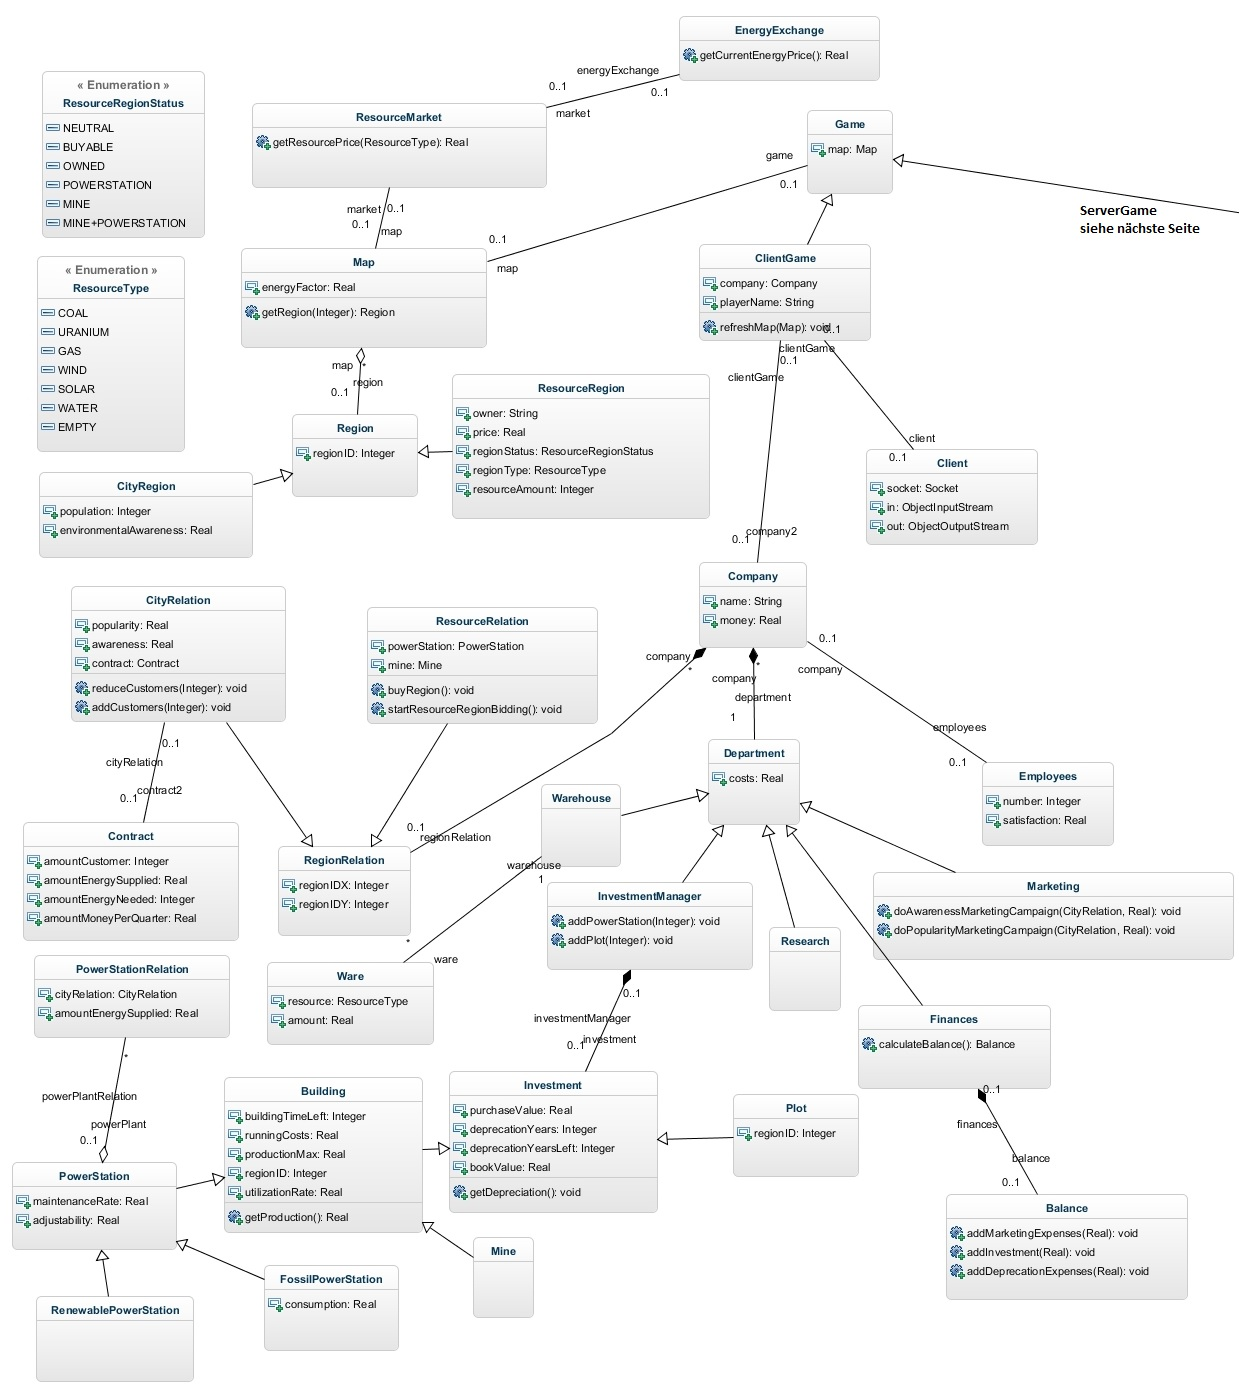
\includegraphics[width=1.3\textwidth]{se-wa-jpg/Client}
\caption{Klassendiagramm Teil 1}
\label{OOA-Client}
\end{figure}
%Die Grafik in Abbildung 
%\ref{labelname} auf Seite \pageref{labelname} ..
\begin{figure}
\centering
\centering
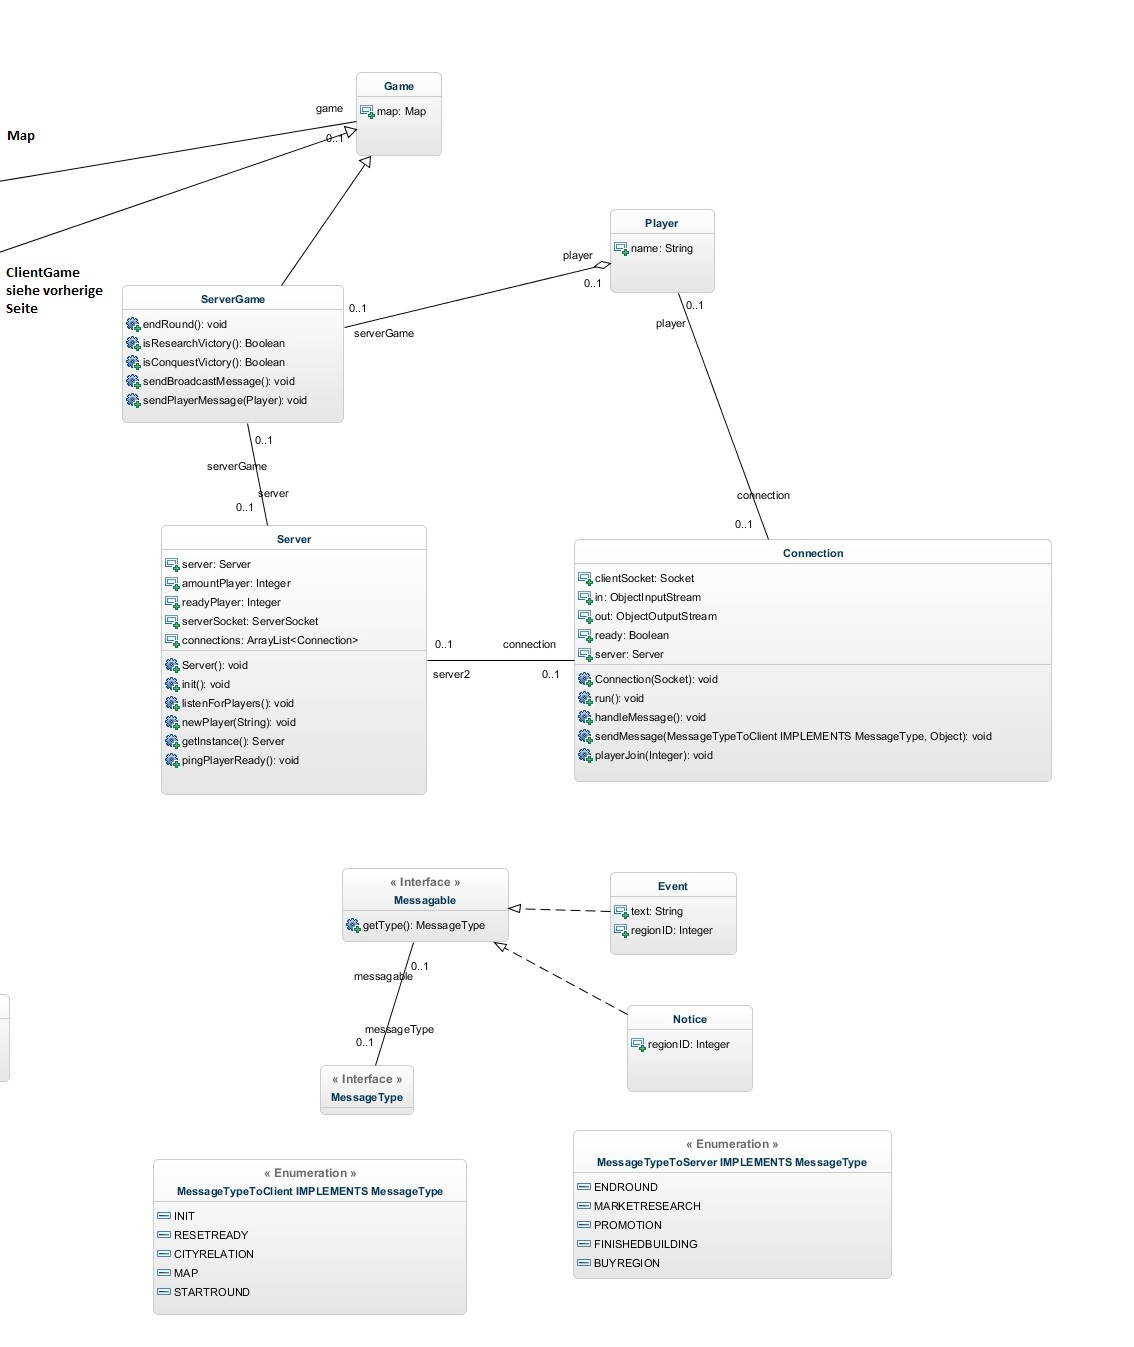
\includegraphics[width=1.1\textwidth]{se-wa-jpg/Server}
\caption{Klassendiagramm Teil 2}
\label{OOA-Server}
\end{figure}


% Anhang der Arbeit
% 
%

% Der Anhang sollte auf einer neuen Seite beginnen; daher wird der Seitenvorschub bei neuen Kapiteln 
% wieder angeschaltet; Achtung: die Verwendung von newpage erzeugt eine Kopfzeile, was dann nicht zu dem 
% Gesamtlayout des Dokuments passt
%
%
\seChaptersNewpage
\seAppendix{}



%
%  Erzeugung eines Glossars
%
% Achtung: Das Glossar wird nur ausgegeben, wenn mindestens ein Eintrag in der Arbeit 
%                definiert wurde
%
%

% Die folgenden Kapitel beginnen jeweils auf einer neuen Seite
%
%
\seChaptersNewpage{}
\newpage
\sePrintGlossary{}


%
% Literaturverzeichnisses
%
%\newpage
\sePrintBibliography{}

%%  Erzeugung von Eintr\"agen im Literaturverzeichnis
%
%  Achtung: in einer Seminar-/Projekt/Bachelorarbeit darf da \nocite-Kommando nicht verwendet werden,
%                 da es einen Eintrag im Literaturverzeichnis erzeugt, ohne dass eine 
%                 entsprechende Literaturreferenz im Text der Arbeit angegeben wird
%
%
%
\nocite{DHBW:SG}
\nocite{KM:KS}
\nocite{Dud06}
\nocite{Dud09}
\nocite{Bri:WA}
\nocite{RP:WA}
\nocite{Sch:WAS}
\nocite{BSS:WA}
\nocite{Kor:WA}
\nocite{MK:GWA}
\nocite{ADG:WA}
\nocite{The:WA}
\nocite{BA:WA}
\nocite{Dij:CRT}
\nocite{BC:Cur}
\nocite{Par:ECP}
\nocite{Bro:SBE}
\nocite{GI:ADI}
\nocite{GI:AZI}
\nocite{Den:CD}
\nocite{LMS:Icb}
\nocite{Fre:SIF}




%
% Festlegung des grundlegenden Formatierungsstils des Literaturverzeichnis
%
\bibliographystyle{jurabib}

% Eigentliche Ausgabe der in der Arbeit verwendeten Quellen
%
%
% Angabe der bib-Dateien, in denen die Quellen beschrieben sind;
% die Angabe geht davon aus, dass eine wa.bib-Datei in demselben 
% Verzeichnis liegt, wie se-ba-vorlage.tex
%

% 2012-02-06
%
% Umbenennung von Literatur- in Quellenverzeichnis
% 
%\renewcommand*{\bibname}{Quellenverzeichnis}
\seBibliography{wa}


%
% Erzeugung der ehrenw\"ortlichen Erkl\"arung
%
% Der optionale Parameter kann verwendet werden, um f\"ur das Thema der Arbeit eine 
% andere Formatierung vorzunehmen; das sollte in der Regel nicht erforderlich sein;
% ausserdem besteht die Gefahr inkonsistenter Titel auf dem Titelblatt und in der 
% ehrenw\"ortlichen Erkl\"arung
%
%\seEhrenwoertlicheErklaerung{} % dieses Kommando sollte standardm\"assig verwendet werden
\seEhrenwoertlicheErklaerung[\LaTeX-Vorlage zur Anfertigung einer Seminararbeit (Version \version{})]


\end{document}











